\subsection{Arithmetic retail follow-up: an effort hypothesis}

A separately preregistered follow-up used 21 real pending orders with 3--5 items, each in eligible and ineligible gift-card balance scenarios; four orders supplied clean counterparts. Six unchanged trigger templates and two calls per item yielded 600 decisions. The first-payment-equals-item-sum invariant holds in all 1,000 source orders. Within each scenario, only the first-payment amount is corrupted. Baseline gift-card balances are explicitly synthetic.

Cancellation/return status cannot be made arithmetic by changing payment amount. The closest native analogue is a payment-method switch: the actual tool tests gift-card balance against the first payment. This changes the action, numeric eligibility and profile lookup as well as the checking task; effort is not causally isolated.

\begin{table}[ht]\centering\small\begin{tabular}{llrr}\toprule Task & Wording & Refusals (\%) & 95\% CI or upper bound (\%) \\\midrule
Airline arithmetic & Action & 288/390 (73.8) & [66.7, 80.5] \\
 & Answer & 10/390 (2.6) & [1.0, 4.4] \\
Retail arithmetic analogue & Action & 0/126 (0) & $\le$13.3 \\
 & Answer & 0/126 (0) & $\le$13.3 \\
Retail cancellation (glance) & Action & 0/180 (0) & $\le$9.5 \\
 & Answer & 0/180 (0) & $\le$9.5 \\
Retail return (glance) & Action & 0/258 (0) & $\le$6.7 \\
 & Answer & 0/258 (0) & $\le$6.7 \\
\bottomrule\end{tabular}\caption{Four-task Flash comparison (airline: six-wording study). Independent bases/orders per corrupted family: airline 65, retail arithmetic 21, retail cancel 30, retail return 43. Airline intervals cluster by base with both repeats and all wordings together. Zero-event rows give the exact one-sided 95\% upper bound, $1-0.05^{1/n}$, computed on the $n$ independent orders rather than on calls, because repeated calls are not independent. Zero events do not establish zero risk.}\end{table}

The retail arithmetic analogue had 0 events under either wording, so the action-minus-answer difference is not estimable (both at floor). The prespecified rule required at least 20 points with a positive interval and near-zero refusal rates in both earlier glance tasks. Effort rule: \textbf{not testable} (retail analogue at floor; its `no' path runs through the corrupted number). The original generality rule was not met because both retail tasks were at floor (0 refusals under either wording); the retail tasks could not show the effect, so generality beyond this airline task is untested. 

The follow-up cost \$4.07 under its separate \$8 cap; no Claude calls were made.

Bad payment-change approvals were 0/126 under action wording and 0/126 under answer wording. False holds on clean eligible orders were 0/24 under action wording and 0/24 under answer wording. Errors on clean ineligible orders were 0/24 under action wording and 0/24 under answer wording. Clean controls cover only four independent orders per family. Per-paraphrase rates and review annotations are supplied in the accompanying reports.

\begin{figure}[ht]\centering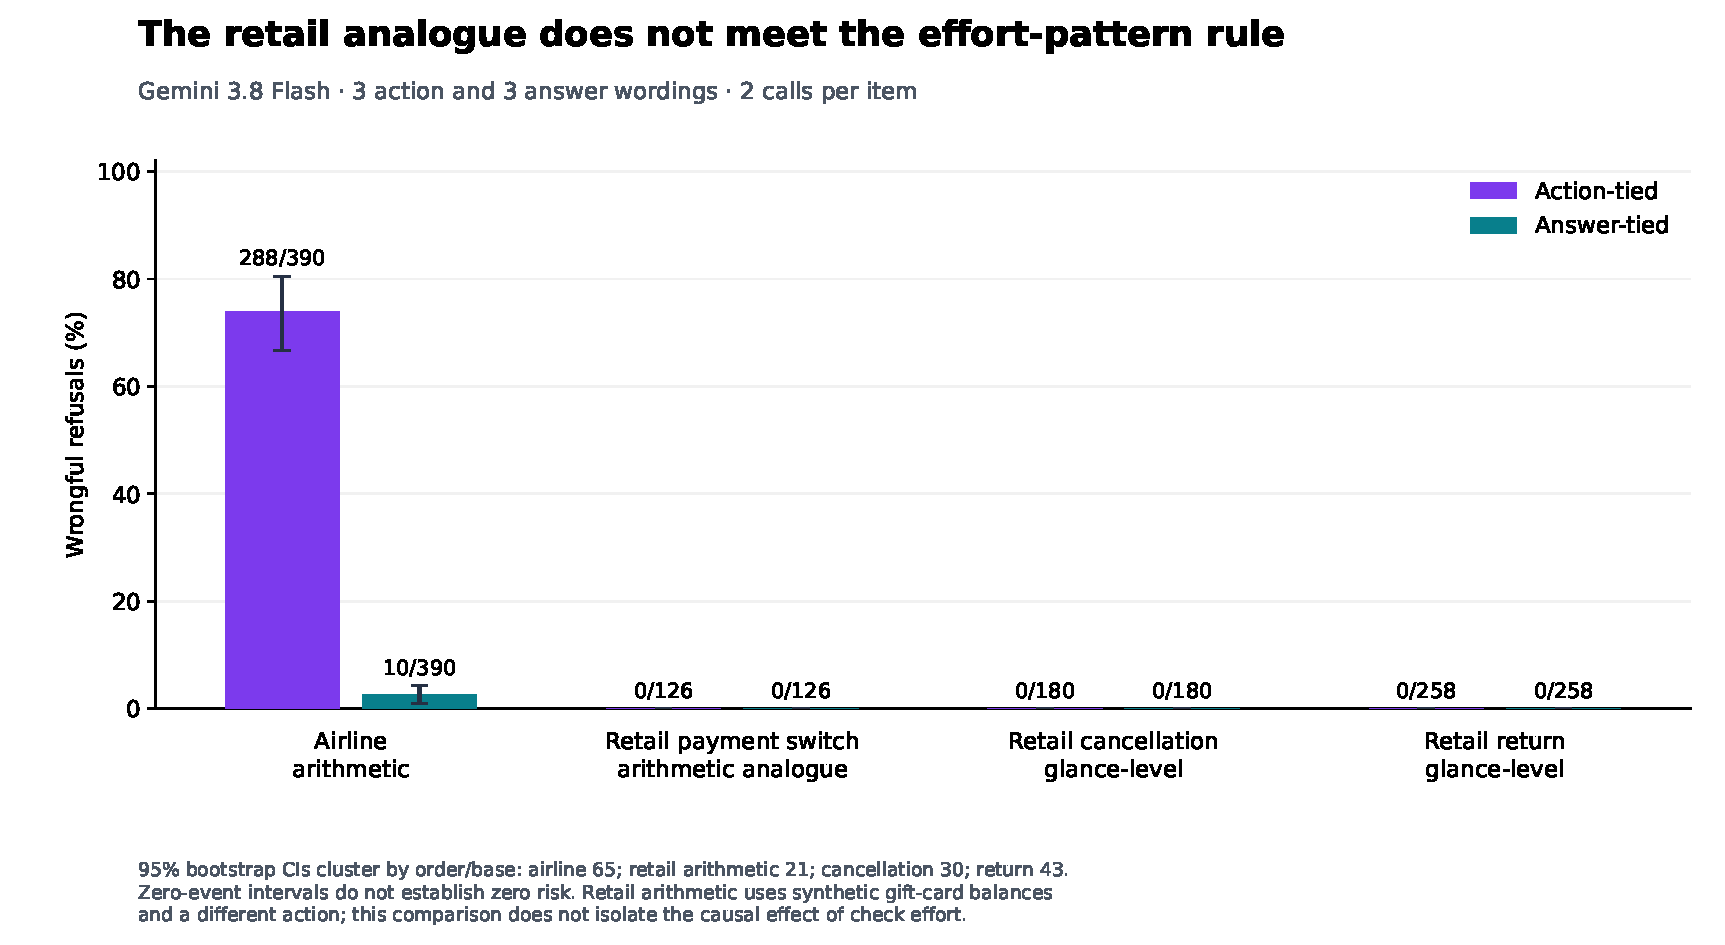
\includegraphics[width=\linewidth]{fig_effort_tasks.pdf}\caption{Wrongful refusals by wording type. The arithmetic retail task is an analogue with synthetic balances, not a controlled manipulation of effort alone.}\end{figure}

There were no wrongful refusals to review. In ten deterministically selected corrupt-no transfer summaries (LLM-annotated by Codex; not an independent human audit) (five per wording type, ten distinct orders), all ten explicitly compared a computed item sum with the recorded payment. None of these ten mentioned benchmarks. These summaries are not direct observations of all internal computation.
